\documentclass[11pt, oneside]{article}   	% use "amsart" instead of "article" for AMSLaTeX format
\usepackage{geometry}                		% See geometry.pdf to learn the layout options. There are lots.
\geometry{letterpaper}                   		% ... or a4paper or a5paper or ... 
%\geometry{landscape}                		% Activate for rotated page geometry
%\usepackage[parfill]{parskip}    		% Activate to begin paragraphs with an empty line rather than an indent
\usepackage{graphicx}				% Use pdf, png, jpg, or eps§ with pdflatex; use eps in DVI mode
								% TeX will automatically convert eps --> pdf in pdflatex		
\usepackage{amssymb}
\usepackage{siunitx}

%SetFonts

%SetFonts


\title{Brief Article}
\author{The Author}
%\date{}							% Activate to display a given date or no date

\begin{document}
\begin{flushright}
Donovan Guelde\\
CSCI 5622\\
Learning HW\\
\end{flushright}
1.  To determine the number of training samples required to find a hypothesis that, with probability 95\%, has an error of at most 0.15, we use the formula $m\geq \frac{1}{\epsilon} (n\ ln(|H|) + ln (\frac{1}{\delta}))$, where:\\
\indent $\epsilon = .15$, $\delta = .05$ and $|H|$ is the number of hypotheses in our hypothesis class.\\
\indent $|H|$ can be determined from the geometry of our hypothesis space, that of all possible triangles with vertexes (i,j) where i,j$\in$ integers in the range [0,99].\\
\indent For each vertex of the triangle, there are (100*100) possible values for (i,j), and there are three vertexes, so the number of hypotheses in our hypothesis class is $(100^2)^3$, or \num{1e12}.\\
\indent Now we have:\\
\indent $m\geq \frac{1}{0.15}(ln(\num{1e12})+ln(\frac{1}{0.05})) = 572.592$\\
\indent To achieve the desired probability and accuracy, we need at least 573 training samples.\\\\\\
2.  Considering the hypothesis class H of linear hyperplanes in 2D that pass through the origin, the lower bound on the VC dimension is 2.  It is possible to shatter a set of two points in the first quadrant with a line passing through the origin, as shown here:\\
\indent\indent 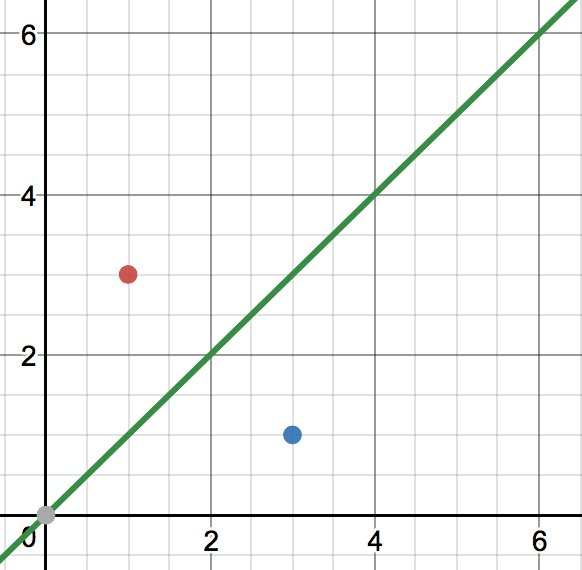
\includegraphics[scale=.4]{shatter}   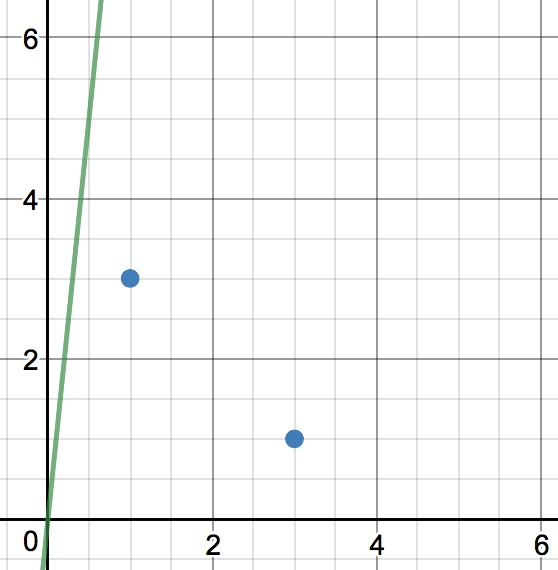
\includegraphics[scale=.20]{shatter2}  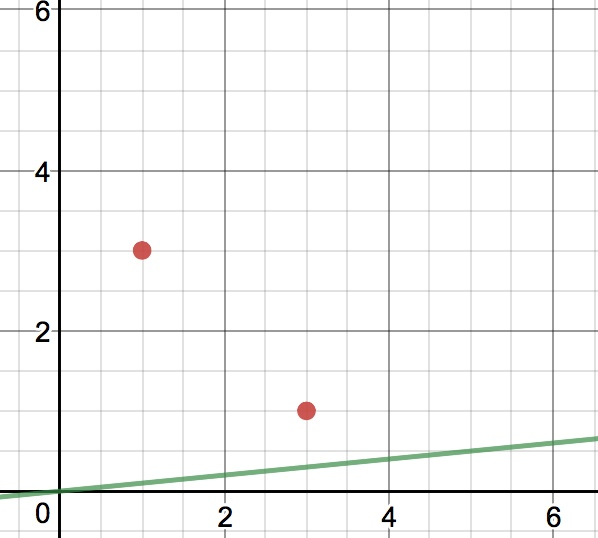
\includegraphics[scale=.20]{shatter3}\\
\indent It appears that the upper bound of this hypothesis class is also 2, but we must prove it.  Do do so, we must show  than no set of points $p_1,p_2,p_3 = (x_1,y_1),(x_2,y_2),(x_3,y_3)$ can be shattered by a line passing through the origin.\\
\indent First, the points $p_1,p_2,$ and $p_3$ are placed anywhere in the first quadrant.  Our classifier, the line passing through the origin, begins at an angle $\theta$ from the origin.  Define our classification scheme as points above the line are labeled as (+), and points below the line are labeled (-).  At $\theta =0$, the line is on the x-axis, and will classify all three points the same (+,+,+).  Now we increase angle $\theta$ until the line crosses one and only one point.  Now, one point is separated from the other two (representing a (+,+,-) classification).  Continuing to increase the angle $\theta$, the line will cross over the second point, $p_2$, resulting in a labelling of (+,-,-).  Again increasing $\theta$ until it crosses the point $p_3$, we have the classification (-,-,-).  Ordered by increasing angle $\theta$ required to achieve the specific classification, we have $(+,+,+) \leq (+,+,-) \leq (+,-,-) \leq (-,-,-)$.  We use $\leq$ in the previous inequality to account for the possibility that two or more points may be colinear relative to our classifying line.\\
\indent These are the only possible outcomes of our classification hypothesis class, since as $\theta$ increases from 0 to $\frac{\pi}{2}$ radians, it is impossible to classify a three-point system via our hypothesis class as (+,-,+) or (-,+,-).  Therefore, the upper bound on the VC dimension is 2, the lower bound is 2, as shown previously, VC dimention is 2.\\\\\\
3.  To calculate the weight $w$ that allows our classification hypothesis $sign(sin(w*\frac{1}{2^{-k}}))$ to shatter any given set of points on the x-axis, it is helpful to recall some fundamental properties of the sin function:\\ 
\indent $sin(\pi x) = -sin(x)$\\
\indent $sin(2\pi x) = sin(x)$ (holds true for any even multiple of $\pi$)\\
\indent $sin(x)$ is positive for all values (0,$\pi$), and negative for all values of i ($\pi$,2$\pi$)\\
\\ To shatter any given set of points $x_1,x_2,...,x_n$ with labels $y_1,y_2,...,y_n$, we can use the following summation to determine weight w:\\
\indent $w = \pi(1+\sum_i^n (1-y_i)(2^{x_i}))$\\
\indent and we use this w in our classifier: $y_i = sign(sin(\frac{w}{2^{k}}))$\\
When the above function is evaluated, $\frac{w}{2^{-k}}$ will be simplified in one of two ways:\\
\indent Case 1:  Where $y_i$ = True:\\
\indent\indent Since all of the terms involved in the summation for determining w are derived from \indent\indent the $y_i=False$ training examples, the term in question will simplify to:\\
\indent\indent\indent  $\frac{\pi}{2^k} + ($some\ multiple\ of\ 2\ *\ $\pi$), giving the classifier as:\\
\indent\indent $sign(sin(\frac{1}{2^z}\pi))$ (where z is come integer $\geq$ 1), which is always positive.\\\\
\indent Case 2: Where $y_i = False$\\
\indent\indent If $y_i = False$, then the term ($\frac{w}{2^k}$) simplifies to:\\
\indent\indent\indent $\frac{\pi}{2^k}$ + $\pi$ + (some multiple of 2* $\pi$), which is always in the range($\pi,2\pi$).\\
\indent\indent This causes the classifier to return (-)\\
\end{document}  